\documentclass[
    a4paper, 
    12pt, 
    twoside,
    % twocolumn
]{article} % A4 paper size, default 11pt font size and oneside for equal margins
% %                                     % , twocolumn
% \usepackage[nochapters, dottedtoc]{classicthesis}

% \usepackage{fancyhdr}

% \pagestyle{fancy}
% \fancyhf{} % clear all headers/footers
% \fancyhead[LE,RO]{\thepage} % page numbers on left even / right odd
% \fancyhead[RE]{\nouppercase{\rightmark}} % section name on even pages
% \fancyhead[LO]{\nouppercase{\rightmark}} % section name on odd pages

% \renewcommand{\sectionmark}[1]{\markright{#1}} % make \rightmark store section name


% \RequirePackage{silence} % :-\
% \WarningFilter{scrreprt}{Usage of package `titlesec'}
% %\WarningFilter{scrreprt}{Activating an ugly workaround}
% \WarningFilter{titlesec}{Non standard sectioning command detected}
% \documentclass[ twoside,openright,titlepage,numbers=noenddot,%1headlines,
% headinclude,footinclude,cleardoublepage=empty,abstract=on,
% BCOR=5mm,paper=a4,fontsize=12pt
% ]{scrreprt}

% \input{classicthesis-config.tex}


% \usepackage[nottoc]{tocbibind}


\usepackage[utf8]{inputenc} % Required for inputting international characters
\usepackage[T1]{fontenc} % Output font encoding for international characters
\usepackage[french, english]{babel}

\selectlanguage{english} 
\usepackage{csquotes}

\usepackage[twoside, margin=2cm, bindingoffset=0.0cm]{geometry}

\usepackage{hyperref} %For hyperlinks 
\hypersetup{pdfborder=0 0 0}

\usepackage{graphicx}  % Pour images
\graphicspath{{Figures/}}
\usepackage{float}
\usepackage{wrapfig}
\usepackage{xcolor}
\usepackage{subfig}
% \usepackage[bottom]{footmisc}
\usepackage{tablefootnote}
\usepackage{enumitem} % for custom item enumeration
% \usepackage{subcaption}
\usepackage{listings}
\lstset{
basicstyle=\small\ttfamily,
columns=flexible,
breaklines=true
}


\usepackage[%backend=biber,
style = ieee,
sorting=none
]{biblatex} %,bibstyle=ieeehttps://www.overleaf.com/project/624dc5f129c1767e8bb8de67
\addbibresource{biblio.bib}
\renewbibmacro*{date}{%
  \iffieldundef{year}
    {\bibstring{nodate}}
    {\printdate}
}

\usepackage{amsmath}
\usepackage{amssymb}
\usepackage{amsthm}
\usepackage{physics} %pour \vb*{b}old vectors
\usepackage{bm}
%\newcommand{\vb*}[1]{\boldsymbol{#1}}
%\newcommand{\vb*}[][]{}

\newcommand{\comment}[1]{}%pour faire des comentaires a plusueures lignes 
\newcommand{\pd}[2]{\frac{\partial #1}{\partial #2}}
\newcommand{\parder}[2]{\frac{\partial #1}{\partial #2}}
\newcommand{\f}[2]{\frac{ #1}{ #2}}
\newcommand{\ol}[1]{\overline{#1}}
% \newcommand{\dd}[1]{\mathrm{d}#1} % TODO trouver une meilleure alternative que ca car ca enleve litalique et apres faire renewcommand \vb*{\}\(
% \newcommand{\of}{OpenFOAM}
% \newcommand{\ofs}{OpenFOAM \space}

\usepackage{xstring}
% \newcommand{\PhilippeDruault}{Philippe Druault}
% \newcommand{\PhilippeDRUAULT}{Philippe DRUAULT}
% \newcommand{\JeanFrancoisKrawczynski}{Jean-François Krawczynski}
\newcommand{\StephaneZaleski}{Stéphane Zaleski}
\newcommand{\StephaneZALESKI}{Stéphane ZALESKI}
\newcommand{\ijlrd}{Institut Jean le Rond $\partial ' \textrm{Alembert}$ \space}
% \newcommand{\MariaIkkenecheu}{Maria Ikkenecheu}
% \newcommand{\PIV}{Particle image velocimetry}
% \newcommand{\LDV}{Laser doppler velocimetry}
% \newcommand{\JeanCamilleChassaing}{Jean-Camille Chassaing}
% \newcommand{\JeanCamilleCHASSAING}{Jean-Camille CHASSAING}
% \newcommand{\RemyCornaggia}{Rémi Cornaggia}
% \renewcommand{\chaptermark}[1]{}

\author{Erdi ÇAN \\ \\ Supervisor: \\ \StephaneZALESKI\\ Internship duration 4.5 months}
\title{TODO}
\date{\today}
\usepackage[absolute,overlay]{textpos} % for positioning

% \usepackage{tracklang}
% \usepackage{glossaries-extra}

% \makeglossaries

% % Define your symbols
% \newglossaryentry{symb:pi}{
%     name={$\pi$},
%     description={The ratio of a circle's circumference to its diameter},
%     sort={pi}
% }

% \newglossaryentry{symb:delta}{
%     name={$\Delta$},
%     description={Difference or change in a quantity},
%     sort={delta}
% }

\begin{document}

\begin{titlepage}
    \centering
    % Include the figure
    % \includegraphics[width=0.9\textwidth]{Figures/Cluster/VAT_U7zoom.png} % replace with your file name

    \vspace{2cm} % space between figure and title
    {\Huge \bfseries Sensitivity Analysis of Initial Conditions In Lagrangian Droplet train simulations.}

    \vspace{1.5cm}
    {\Large By Erdi ÇAN for Melisa HASGÜL \par}
    \vspace{0.5cm}
    % {\large Supervisors: \\ Jean-François Krawczynski \\ Philippe Druault\par}
% \vspace{0.5cm}
%     {\large Internship duration 3.5 months(May 5-August 29) \par}
    
    % \vfill
    % {\large September 1, 2025 \par}

    \begin{textblock*}{5cm}(15cm,26cm)
      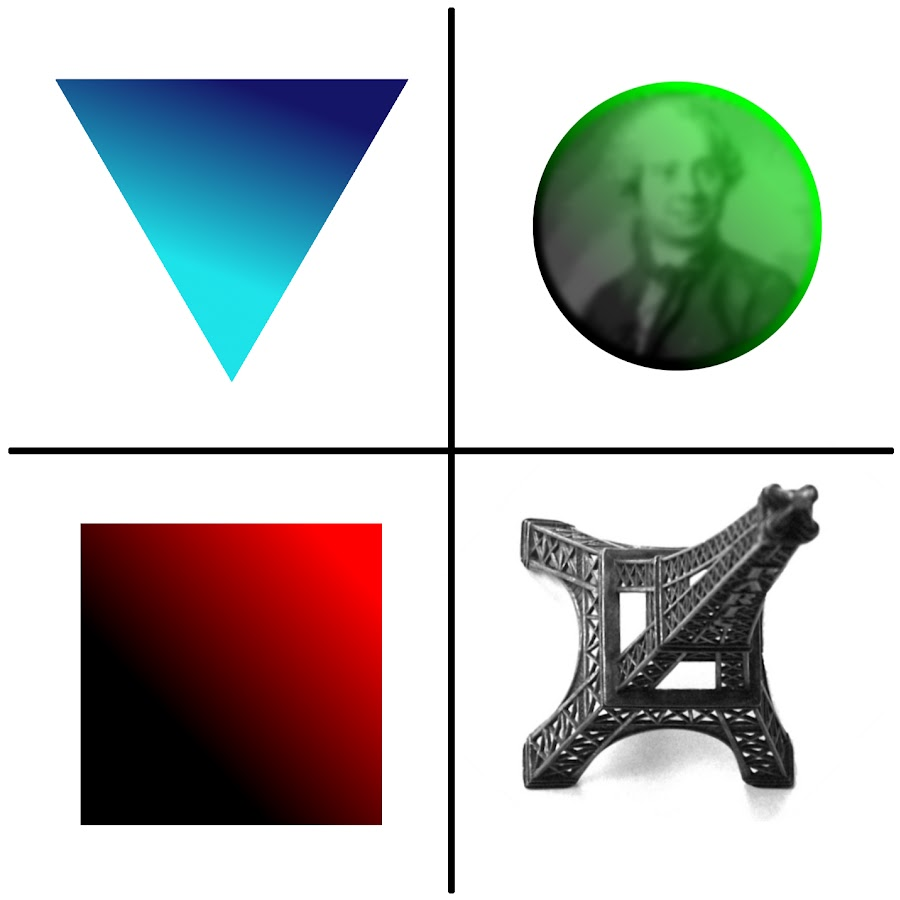
\includegraphics[height=2cm]{Figures/Logos/institut_square_logo.jpg} % replace with your image
    \end{textblock*}
    
    % Bottom-right figure
    \begin{textblock*}{5cm}(1cm,26cm) % {block width} (x,y position)
        
\includegraphics[height=2cm]{Figures/Logos/SORBONNE_FAC_SCIENCES_DEF_CMJN.png} % replace with your image
    \end{textblock*}
    \thispagestyle{empty}
\end{titlepage}
% \maketitle
\newpage
% \thispagestyle{empty}
\pagenumbering{arabic}
\section{Introduction}
\begin{figure}[H]
    \centering
    \includegraphics[width=\textwidth]{/home/erdi/Uni/LCGAStage/Presentations/MajorPresentation/Figures/exp_bonn.png}
    \caption{Figure taken from \cite{jets_and_sprays}}
    \label{bonn_exp}
\end{figure}

After the experiences of Stefan Kooji et. al.\parencite{jets_and_sprays} (shown in figure \ref{bonn_exp}) made in Amsterdam they find out that the droplet statistics after the Rayleigh-Plateau instability took the form of a Frachebourg distribution \cite{FrachebourgL.1999ESot}. And their main conclusion is that droplets have a ballistic colisions and that everything can be explained by the ballistic theory \cite{jets_and_sprays} \cite{statistics_of_balistic_agglomeration}. There for I have coded a Lagrangian droplet simulator that takes as input the droplet velocity distributions and the droplet diameter distributions and every time interval it selects a droplet to inject then takes a droplet diameter and velocity according to the distributions in the experiments that can be seen in the figure \ref{exp_init_lin}.          

\begin{figure}[H]
    \centering
    
\includegraphics[width = 0.49\textwidth]{exp11mm_vel_pdf_lin_lin.pdf}
    
\includegraphics[width = 0.49\textwidth]{exp11mm_dia_pdf_lin_lin.pdf}
    \caption{Experimental velocity(left) and diameter(right) probability distributions. Coloured by if the droplet is a satelite(orange) or main(blue) droplet. In lin-lin plotting.}
    \label{exp_init_lin}
\end{figure}

\section{How to run the program}
The program is not the most polished program there for you might need some nuances to navigate through it. It uses the make compilation tool with a makefile. In that make file it is important to put the correct paths MAT\_NUM\_INC and LAGJET\_INC\_DIR\_SRC and there it need to be the directories corresponding to the Include paths of each respectively. 

Then once everything is setup in the makefile inside the LagrangianJet directory you can run "make" in the terminal and it should compile the program. Once the program is compiled you can try to run the program in the command line using: 

\begin{lstlisting}
    ./exe.exe TestFolder/Standart dt=0.01 injection_rate=29.25 recording_distance_in_mm=111 nb_droplets_saved=1000
\end{lstlisting}

Now normaly the program should run without any errors if there are any errors come see me please.


\section{Tasks}
\begin{enumerate}%[label=\textbf{Question \arabic*.}]
    \item Plot the volume weighted PDF for the 11mm and 111mm cases in the same figure one in lin-log and the other in lin-lin.
    \item Convert the experimental volume weighted probability densities to non weighted probability densities. Both for the 11mm and 111mm. The x axis it the L111mmdia\_x which is what diameter corresponds to the volume weighted PDF in L111mmdiaPDFByVolume\_y. Likewise for the 11mm.  
    \item Plot the experimental non weighted PDFs that you found in the previous question. 
    \item From the theory find the Rayleigh-Plateau droplet formation frequency or time interval at 11mm from a jet that is started from a nozzle of diameter $64\mu m $ and a velocity of $10.15 m/s$. (The answer is 29.25 but need the handwritten proof). 
    \item Now that we know our inputs run the program with experimental setup for 100000 droplets saved with an injection rate of $29.25 \mu s$ and with a $dt = 0.01$ how does the distribution look like at 11mm and 111mm?   
\end{enumerate}

\newpage
% \thispagestyle{empty}
\pagenumbering{roman}
\nocite{*}
\addcontentsline{toc}{section}{Bibliography}
\printbibliography[title = Bibliography]

\end{document}